\documentclass[11pt]{article}
\usepackage[utf8]{inputenc}
\usepackage[T1]{fontenc}
\usepackage{amsmath}
\usepackage{amssymb}
\usepackage{multicol}
\usepackage{geometry}
\usepackage{tikz}
\usepackage{enumitem}
\usepackage{xcolor}
\usepackage{titlesec}

% Configurações de layout
\geometry{a4paper, left=1cm, right=1cm, top=0.5cm, bottom=1.2cm}
\setlength{\columnseprule}{0.4pt}

% Cores para títulos
\titleformat{\section}{\normalfont\Large\bfseries\color{blue}}{\thesection}{1em}{}
\titleformat{\subsection}{\normalfont\large\bfseries\color{red}}{\thesubsection}{1em}{}

\title{\textcolor{orange}{Terceiro Trimestre: Matemática
    \\Progressão Aritmética - Revisão}}
\author{Professor: Jefferson}
\date{}

\begin{document}

\maketitle
\vspace{-1cm}

\begin{center}
\large{Nome: \underline{\hspace{8cm}} \quad Turma: \underline{\hspace{3cm}}}
\end{center}

\begin{multicols}{2}

\section*{Fórmulas Importantes}

\subsection*{Termo Geral da PA}

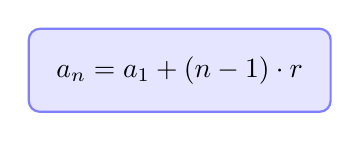
\begin{tikzpicture}
\node[rectangle, fill=blue!10, rounded corners, inner sep=10pt, draw=blue!50, thick] (box) {
$\displaystyle a_n = a_1 + (n-1) \cdot r$
};
\end{tikzpicture}

\textbf{Onde:}
\begin{itemize}
\item $a_n$ = termo que queremos
\item $a_1$ = primeiro termo
\item $n$ = posição do termo
\item $r$ = razão (diferença entre termos)
\end{itemize}

\subsection*{Razão da PA}

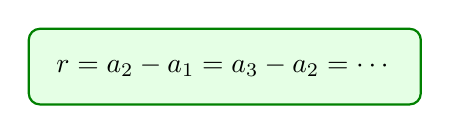
\begin{tikzpicture}
\node[rectangle, fill=green!10, rounded corners, inner sep=10pt, draw=green!50!black, thick] (box) {
$\displaystyle r = a_2 - a_1 = a_3 - a_2 = \cdots$
};
\end{tikzpicture}

\subsection*{Soma dos Termos}

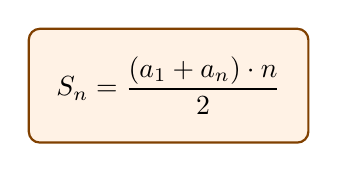
\begin{tikzpicture}
\node[rectangle, fill=orange!10, rounded corners, inner sep=10pt, draw=orange!50!black, thick] (box) {
$\displaystyle S_n = \frac{(a_1 + a_n) \cdot n}{2}$
};
\end{tikzpicture}

\section*{Exercícios Básicos}

\begin{enumerate}[leftmargin=*]

\item Determine a razão de cada PA:
\begin{enumerate}[label=\alph*)]
\item $(2, 5, 8, 11, \ldots)$
\item $(10, 7, 4, 1, \ldots)$
\item $(-3, 1, 5, 9, \ldots)$
\end{enumerate}

\item Calcule o 5º termo de cada PA:
\begin{enumerate}[label=\alph*)]
\item $(4, 7, 10, 13, \ldots)$
\item $(15, 12, 9, 6, \ldots)$
\item $(1, 4, 7, 10, \ldots)$
\end{enumerate}

\item Encontre o 10º termo das PAs:
\begin{enumerate}[label=\alph*)]
\item $(2, 6, 10, 14, \ldots)$
\item $(20, 17, 14, 11, \ldots)$
\end{enumerate}

\item Escreva os 4 primeiros termos da PA sabendo que:
\begin{enumerate}[label=\alph*)]
\item $a_1 = 3$ e $r = 4$
\item $a_1 = 10$ e $r = -2$
\item $a_1 = -5$ e $r = 3$
\end{enumerate}

\item Calcule a soma dos:
\begin{enumerate}[label=\alph*)]
\item 6 primeiros termos da PA $(1, 3, 5, 7, \ldots)$
\item 8 primeiros termos da PA $(2, 5, 8, 11, \ldots)$
\item 5 primeiros termos da PA $(10, 8, 6, 4, \ldots)$
\end{enumerate}

\item Interpole 3 meios aritméticos entre:
\begin{enumerate}[label=\alph*)]
\item 2 e 10
\item 5 e 17
\end{enumerate}

\item Problemas simples:
\begin{enumerate}[label=\alph*)]
\item Uma PA tem $a_1 = 4$ e $r = 3$. Qual é o 8º termo?
\item Uma PA tem $a_1 = 20$ e $r = -2$. Qual é o 6º termo?
\item Calcule a soma dos 10 primeiros termos da PA $(1, 4, 7, 10, \ldots)$
\end{enumerate}

\item Complete as PAs:
\begin{enumerate}[label=\alph*)]
\item $( \_, 5, 8, 11, \_ )$
\item $(10, \_, 4, \_, -2)$
\item $( \_, 7, 11, 15, \_ )$
\end{enumerate}

\item Determine o número de termos das PAs:
\begin{enumerate}[label=\alph*)]
\item $(3, 7, 11, \ldots, 43)$
\item $(20, 18, 16, \ldots, -10)$
\end{enumerate}

\item Problemas do cotidiano:
\begin{enumerate}[label=\alph*)]
\item João guarda R\$ 5,00 no 1º dia, R\$ 8,00 no 2º dia, R\$ 11,00 no 3º dia, e assim por diante. Quanto guardará no 10º dia?
\item Uma escada tem degraus com alturas em PA: 20 cm, 25 cm, 30 cm... Qual a altura do 8º degrau?
\end{enumerate}

\end{enumerate}

\section*{Dicas para Resolver}

\begin{itemize}
\item \textbf{Razão}: Sempre subtraia um termo pelo anterior
\item \textbf{Termo geral}: Use $a_n = a_1 + (n-1) \cdot r$
\item \textbf{Soma}: Some primeiro + último, multiplique por n e divida por 2
\item \textbf{Verificação}: Confira se a diferença entre termos é constante
\end{itemize}

\end{multicols}

\end{document}
